\documentclass[conference]{IEEEtran}
\usepackage{graphicx}
\usepackage{booktabs}
\usepackage{amsmath}
\usepackage{array}
\usepackage{url}
\usepackage[hidelinks,pdfauthor={Anonymous},pdftitle={Empirical Multi-Feature Model Development and Genetic Decision Optimization for Cross-Platform Identity Resolution},pdfsubject={Anonymous conference submission}]{hyperref}

\title{Empirical Multi-Feature Model Development and Genetic Decision Optimization for Cross-Platform Identity Resolution}
\author{\IEEEauthorblockN{Anonymous Submission}}

\begin{document}
\maketitle

\begin{abstract}
Cross-platform identity resolution is both an evidence-integration problem and an operational decision problem. Fragmented profiles provide heterogeneous, incomplete clues; even a calibrated match probability does not specify whether an automated system should merge, defer, or reject a pair. We connect two empirical development stages: a multi-feature Gradient Boosting pair scorer and genetic optimization of a three-way MATCH/REVIEW/NO\_MATCH policy under a declared remediation-effort objective. The final controlled study compares a 17-feature model with a semantic-augmented variant, then separates fixed operation, validation tuning, policy-class expansion, and optimizer choice. Three entity-disjoint outer partitions use physically sealed test labels and equal 12,000-evaluation Sobol/genetic budgets. Validation tuning raises decision-conditional F1 from 0.8510 to 0.8910, but automatic end-to-end F1 rises only from 0.8420 to 0.8667; review increases from 0.0871\% to 0.3847\% of candidates. Objective loss falls from 2364.2 to 1864.6. The expanded genetic policy reaches loss 1858.2 versus 1860.0 for equal-budget Sobol and 1879.0 for a direct posterior-risk reject rule. These small empirical differences do not establish optimizer superiority. Candidate retrieval covers 25,931 of 29,243 cross-platform positives (88.6742\%), bounding end-to-end recall. The evaluation concerns pairwise linkage decisions, not human review outcomes or entity clustering.
\end{abstract}

\section{Introduction}
A person's online identity is often split across platforms. Usernames drift, biographies are incomplete, and the same field follows different platform conventions. Linking these fragments requires two different capabilities. First, a model must combine heterogeneous evidence to estimate whether two profiles belong to one entity. Second, an operating policy must decide how to act when evidence is uncertain and mistakes have asymmetric consequences.

Research on user identity linkage combines profile, behavioral, and network evidence \cite{shu2017uilreview,linkSocial2018,yao2023profile}. In a profile-only setting, no single field is consistently reliable: names can vary, biographies can be semantically related without lexical overlap, and metadata may be missing. Development-stage experiments therefore motivated an empirical model choice and a multi-feature representation rather than an arbitrary classifier (Section~\ref{sec:representation}, Fig.~\ref{fig:model_family}). Yet the resulting score is still not an action. A fixed cutoff can create false merges, missed merges, or a large uncertain review queue, which in turn motivated scenario-based policy selection.

Fig.~\ref{fig:pipeline} orients the reader to the overall workflow. Earlier entity-disjoint development experiments compared model families and selected Gradient Boosting as the pair scorer. The authoritative experiment then freezes the scorer, adds calibration, and evaluates four increasingly flexible operating strategies: a fixed policy, validation-tuned thresholds, an expanded four-parameter policy searched by Sobol points, and the same policy searched by a genetic algorithm (GA). The policy objective is a transparent scenario-based remediation-effort proxy, not measured financial loss.

The study evaluates two components: (1) an empirically developed multi-feature identity-matching pipeline, including a controlled semantic-feature ablation; and (2) a controlled evaluation of genetic optimization for three-way operational decisions. The ablation separates what comes from validation tuning, added policy flexibility, and optimizer choice. A leakage-safe protocol physically seals test labels, candidate-generation recall bounds the achievable ceiling (Fig.~\ref{fig:ceiling}), and workflow metrics include positives lost in candidate generation.

\begin{figure}[t]
\centering
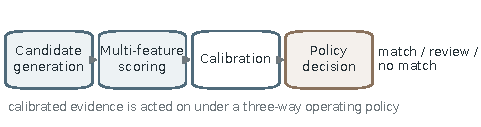
\includegraphics[width=\columnwidth]{figures/system_pipeline.pdf}
\caption{Overall workflow: candidate generation, multi-feature scoring, calibration, and a three-way decision policy.}
\label{fig:pipeline}
\end{figure}

\section{Related Work}
\textbf{Identity linkage and representation.} Fellegi--Sunter linkage introduced match, possible-match, and non-match regions \cite{fellegi1969theory}. Cross-network user linkage extends this setting to heterogeneous social profiles \cite{shu2017uilreview,linkSocial2018}. Neural entity matching and pretrained language models can capture semantic evidence beyond string similarity \cite{barlaug2021survey,li2020ditto}. Our contribution is not a new classifier or embedding; it is the controlled integration of empirical feature/model development with downstream operating-policy selection.

\textbf{Retrieval and abstention.} Blocking controls quadratic comparison cost, but a downstream scorer cannot recover a missed pair \cite{papadakis2021blocking,thirumuruganathan2021deepblocker}. Three-way linkage and reject-option learning explicitly retain uncertainty rather than forcing a binary decision \cite{ouyang2019threeway,chow1970reject,hendrickx2024reject}. Our REVIEW label is an offline system decision; we do not evaluate reviewers.

\textbf{Evolutionary policy search.} GA-based entity-resolution work exists \cite{sun2017gaer}. We therefore make no broad novelty claim for genetic search. Instead, we compare GA with deterministic Sobol search using an identical four-parameter policy, validation data, bounds, objective, and realized evaluation budget.

\section{Evidence and Model Development}
\subsection{Candidate Generation}
We use a normalized local derivative of the public LinkSocial corpus spanning Twitter, Google+, and Instagram \cite{linkSocial2018}. Frozen validity rules retain 36,804 profiles. The eligible cross-platform universe contains 449,149,239 pairs and 29,243 positive links. Deterministic candidate generation yields 12,403 exact-tier pairs and 2,073,842 model-scored pairs, or 2,086,245 workflow candidates. It covers 25,931 positives and misses 3,312, for retrieval recall of 88.6742\% and candidate-space reduction of 99.5355\%. Four same-platform positives are excluded from this denominator. Fig.~\ref{fig:ceiling} shows this split: a downstream scorer cannot recover a pair that candidate generation never presents to it, so the 3,312 missed positives set a hard ceiling on end-to-end recall regardless of classifier quality.

\begin{figure}[t]
\centering
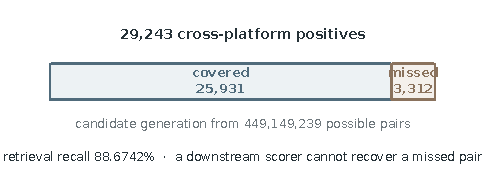
\includegraphics[width=0.72\columnwidth]{figures/candidate_ceiling.pdf}
\caption{Candidate-generation retrieval ceiling over the 29,243 cross-platform positives.}
\label{fig:ceiling}
\end{figure}

\subsection{Empirical Model-Family Choice}
Gradient Boosting was not selected by convention alone. An earlier entity-disjoint development screen compared three families on a 22-feature configuration (Fig.~\ref{fig:model_family}). Validation average precision was 0.9783 for Gradient Boosting, 0.9769 for Random Forest, and 0.9404 for logistic regression, motivating the selected family. These values are historical development evidence only: their feature schema, sampling, and split protocol differ from the final experiment, so they are not used as authoritative test results or combined with Table~\ref{tab:results}.

\begin{figure}[t]
\centering
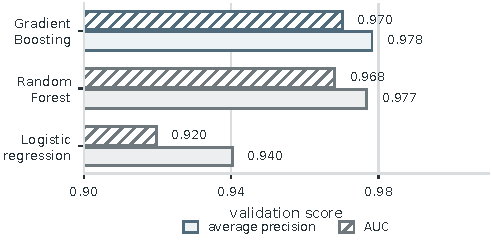
\includegraphics[width=0.85\columnwidth]{figures/model_family_development.pdf}
\caption{Development-stage model-family screen (22-feature configuration, not authoritative V2 evidence).}
\label{fig:model_family}
\end{figure}

\subsection{Multi-Feature Representation}\label{sec:representation}
The broader development program considered identity evidence from usernames, full names, biographies, URL/domain fields, locations, platform context, evidence availability, lexical similarities, and semantic text. The authoritative 17-feature Gradient Boosting model (GB-17) freezes the compatible subset: Jaro, normalized Levenshtein, and token-sort scores for usernames and full names; an unconditional maximum cross-field name similarity; biography Jaccard, length ratio, and availability; location similarity, exactness, and availability; platform agreement; and name length, word-count, and prefix indicators. Missing evidence is encoded deterministically and no feature reads labels, split roles, predecessor scores, or policy decisions.

The semantic-augmented Gradient Boosting model (GB-18) adds exactly one feature: cosine similarity between normalized all-MiniLM-L6-v2 embeddings of profile text assembled from full name, biography, and location. The encoder is fixed and receives no task labels. Thus GB-17 versus GB-18 isolates this semantic cosine; it does not evaluate a general transformer architecture or the full historical feature pool.

For each outer partition, both models use 300 estimators, learning rate 0.05, maximum depth 6, and random state 42. TRAIN retains all positives and a deterministic 3:1 negative sample. An isotonic regressor fitted only on CALIBRATION maps pair scores to $P(\mathrm{match})$ \cite{niculescu2005calibration}.

\section{Three-Way Decision-Policy Selection}
\subsection{From Probability to Operational Action}
The initial policy maps calibrated probabilities to MATCH, REVIEW, or NO\_MATCH with fixed thresholds $t_m=0.98$ and $t_r=0.95$. Earlier fixed-policy experiments exposed the reason for optimization: changing thresholds redistributes uncertain cases among review, false merges, and missed merges. Optimizing classifier discrimination alone cannot choose this operating trade-off.

We use a declared remediation-effort scenario: an erroneous merge costs twice a missed merge, while REVIEW costs one tenth of a missed merge, independently of the label. Correct automated decisions cost zero. The resulting loss is
\begin{equation}
U=2\,FP+FN+0.1\,REVIEW .
\end{equation}
These coefficients are design assumptions, not measured economic costs. REVIEW incurs its declared cost but is not assumed to recover a positive link.

\subsection{Controlled Policy Ladder}
The fixed policy (B0) uses $(t_m,t_r)=(0.98,0.95)$. The validation-tuned simple policy (B1) selects the same rule on policy-validation data:
\begin{equation}
a_{\rm simple}(p)=\begin{cases}
\mathrm{MATCH},&p\ge t_m,\\
\mathrm{REVIEW},&t_r\le p<t_m,\\
\mathrm{NO\_MATCH},&p<t_r.
\end{cases}
\end{equation}
B1 scales Sobol points to $[0.90,0.999]\times[0.50,0.999]$ and sorts each threshold pair so $t_r\le t_m$.

The expanded Sobol policy (B2) and genetic policy (B3) use $\theta=(t_m,t_r,c_p,c_d)$ and a second input $s\in[0,1]$. Here $s$ is the maximum Jaro--Winkler similarity across the four comparisons between each profile's normalized username and full name. Empty fields are excluded; $s=0$ if no comparison is available. Name normalization applies NFKC, case folding, trimming, leading-@ removal, and whitespace collapse. With $p\in[0,1]$ the isotonic-calibrated GB-18 score, the complete rule is
\begin{equation}
\label{eq:expanded}
a_\theta(p,s)=\begin{cases}
\mathrm{MATCH},&p\ge t_m,\\
\mathrm{NO\_MATCH},&p<t_r,\\
\mathrm{MATCH},&t_r\le p<t_m,\ s\ge c_p,\\
\mathrm{NO\_MATCH},&t_r\le p<t_m,\ s<c_d,\\
\mathrm{REVIEW},&t_r\le p<t_m,\ c_d\le s<c_p.
\end{cases}
\end{equation}
Search bounds are $t_m\in[0.90,0.999]$, $t_r\in[0.50,0.90]$, $c_p\in[0.50,1]$, and $c_d\in[0,0.60]$. Proposal repair clips $t_r$ to at most $t_m$ and $c_d$ to at most $c_p$. Thus equality at $t_m$ matches, equality at $t_r$ enters the band, equality at $c_p$ promotes, and equality at $c_d$ does not demote. If $c_d=c_p$, the REVIEW region is empty. These are name-based promotion/demotion thresholds, not additional learned models. B1 and B2 are not strictly nested search domains.

\subsection{Direct Posterior-Risk Baseline}
For the same cost function, the action risks are
\begin{align}
R(\mathrm{NO\_MATCH}\mid p)&=p,\\
R(\mathrm{REVIEW}\mid p)&=0.1,\\
R(\mathrm{MATCH}\mid p)&=2(1-p).
\end{align}
The closed-form reject baseline chooses the minimum-risk action \cite{chow1970reject}. It rejects for $p\le0.1$, reviews for $0.1<p\le0.95$, and matches for $p>0.95$, with ties resolved in the order NO\_MATCH, REVIEW, MATCH. Implementation directly minimizes the three machine-precision risks. It uses the same frozen GB-18 probabilities and no fitting or test-set tuning. Exact-tier MATCH decisions and blocking-missed positives are identical across methods. Its risk optimality assumes the calibrated score is the true posterior; isotonic fitting alone does not guarantee this.

This ladder gives three contrasts: B0--B1 measures validation selection within the simple-policy domain; B1--B2 measures the transition from the tuned simple policy to the declared expanded four-parameter policy and search domain; B2--B3 isolates optimizer choice under an identical policy class, bounds, objective, validation data, and budget. B2 and B3 receive exactly 12,000 realized objective evaluations per outer partition. The GA uses a population of 60 with seeded selection and Gaussian mutation over 200 evaluated populations; proposals are not deduplicated, so it evaluates 8,414/8,488/8,874 unique parameter vectors (seeds 101/202/303) within the equalized call budget, while Sobol evaluates 12,000 distinct points. Only POLICY\_VALIDATION labels guide selection.

\begin{table}[t]
\caption{Controlled decision-policy ladder.}
\label{tab:policies}
\centering
\begin{tabular}{llllr}
\toprule
ID & Descriptive policy & Params. & Search & Eval.\\
\midrule
B0 & Fixed simple & 0 & None & 0\\
B1 & Validation-tuned simple & 2 & Sobol & 12k\\
B2 & Expanded Sobol & 4 & Sobol & 12k\\
B3 & Expanded genetic & 4 & GA & 12k\\
Chow & Direct posterior risk & 0 & None & 0\\
\bottomrule
\end{tabular}
\end{table}

\section{Leakage-Safe Experimental Design}
Each seed (101, 202, 303) assigns complete entities to TRAIN, CALIBRATION, POLICY\_VALIDATION, or SEALED\_TEST. Cross-role pairs are discarded, giving zero entity overlap. Development labels are role-specific. SEALED\_TEST labels reside in separate artifacts and are unavailable during training, calibration, policy selection, and test prediction.

As Table~\ref{tab:roles} shows, label-free test predictions are canonicalized and SHA-256 hashed into a pre-label freeze manifest after models, calibrators, and policies are frozen and before any test-label access; final evaluation refuses to start without this manifest and re-verifies the prediction hash afterwards. Pre-final validation inspects sealed-label artifacts only by content hash, parquet schema, row count, and label-free pair keys; the ground-truth column is materialized solely inside FINAL\_EVALUATION through a single lazy adapter joined by safe pair key. Process-wide runtime instrumentation records zero pre-final test-label-value materializations for all runs. Independent evaluation recomputes row-level decisions and metrics.

\begin{table}[t]
\caption{Entity-disjoint roles and label availability.}
\label{tab:roles}
\centering
\setlength{\tabcolsep}{3pt}
\begin{tabular}{p{0.24\columnwidth}p{0.36\columnwidth}p{0.24\columnwidth}}
\toprule
Role & Used for & Labels\\
\midrule
Train & GB-17 / GB-18 fitting & yes\\
Calibration & isotonic $P(\mathrm{match})$ & yes\\
Policy val. & B1--B3 threshold search & yes\\
Sealed test & final metrics only & frozen\\
\bottomrule
\end{tabular}
\end{table}

Workflow metrics combine exact-tier MATCH decisions, model-scored candidates, and blocking-missed positives assigned NO\_MATCH. Let $TP$ and $FP$ count positive and negative MATCH decisions, $FN$ count positive NO\_MATCH decisions including blocking misses, and $R_+$ count positive REVIEW decisions. REVIEW is neither an automated match nor an evaluated human correction. We preserve the original conditional metrics and add automatic end-to-end metrics:
\begin{align}
P&=\frac{TP}{TP+FP},\quad R_{\rm dec}=\frac{TP}{TP+FN},\\
R_{\rm auto}&=\frac{TP}{TP+FN+R_+},\\
F_{\rm dec}&=\frac{2TP}{2TP+FP+FN},\\
F_{\rm auto}&=\frac{2TP}{2TP+FP+FN+R_+}.
\end{align}
Decision recall excludes deferred positives; it is not end-to-end recall. A zero denominator gives zero. Review rate is REVIEW divided by the number of evaluated exact-tier plus model-scored candidates; coverage is one minus this rate. Blocking misses affect recall and loss but are not reviewable candidates. Ungenerated negative pairs are not included. We aggregate per-partition metrics with equal weights and sample SD, not a pooled confusion matrix. Full per-seed counts, SDs, and optimizer vectors accompany the reproducibility package.

\section{Results and Discussion}
\begin{figure}[!t]
\centering
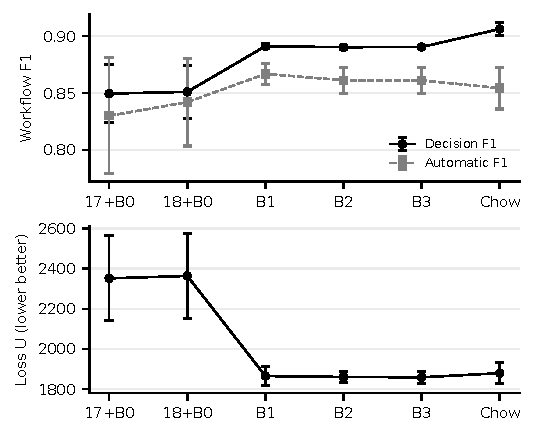
\includegraphics[width=\columnwidth]{figures/controlled_results.pdf}
\caption{Decision-conditional and automatic end-to-end F1, and declared loss, from the same frozen workflow rows. The direct-risk baseline trades greater review for lower false-negative burden.}
\label{fig:results}
\end{figure}

\begin{table*}[t]
\caption{Workflow means over three entity-disjoint partitions. $R_{\rm dec},F_{\rm dec}$ exclude positive REVIEW; $R_{\rm auto},F_{\rm auto}$ retain them. Review rate uses candidate counts. Lower $U$ is better; per-partition results and sample SD are retained in the reproducibility package.}
\label{tab:results}
\centering
\begin{tabular}{lrrrrrrr}
\toprule
Method & $P$ & $R_{\rm dec}$ & $R_{\rm auto}$ & $F_{\rm dec}$ & $F_{\rm auto}$ & Review (\%) & $U$\\
\midrule
GB-17+B0 & 0.9863 & 0.7466 & 0.7187 & 0.8494 & 0.8300 & 0.1884 & 2352.0\\
GB-18+B0 & 0.9870 & 0.7486 & 0.7357 & 0.8510 & 0.8420 & 0.0871 & 2364.2\\
GB-18+B1 & 0.9834 & 0.8146 & 0.7748 & 0.8910 & 0.8667 & 0.3847 & 1864.6\\
GB-18+B2 & 0.9844 & 0.8124 & 0.7654 & 0.8901 & 0.8611 & 0.4273 & 1860.0\\
GB-18+B3 & 0.9844 & 0.8127 & 0.7653 & 0.8903 & 0.8610 & 0.4318 & 1858.2\\
GB-18+Chow & 0.9859 & 0.8384 & 0.7540 & 0.9061 & 0.8542 & 2.0442 & 1879.0\\
\bottomrule
\end{tabular}
\end{table*}

\textbf{What feature development contributed.} Under fixed operation, adding the MiniLM cosine changes mean decision-conditional F1 from $0.8494\pm0.0257$ to $0.8510\pm0.0235$, while $U$ worsens by 12.2. The single semantic augmentation therefore provides no substantive improvement relative to between-partition variation. This comparison does not establish why the semantic addition fails to help, and it does not evaluate other semantic representations.

\textbf{Validation tuning and abstention.} B0 to B1 raises mean decision recall from 0.7486 to 0.8146 and decision F1 from 0.8510 to 0.8910. Automatic recall rises from 0.7357 to 0.7748 and automatic F1 from 0.8420 to 0.8667, a smaller gain. Review rate increases from 0.0871\% to 0.3847\% (coverage falls from 99.9129\% to 99.6153\%). Mean positive REVIEW grows from 160.7 to 430.0. The loss falls by 499.6, with 613.7 fewer FN but 27.3 more FP and 593.7 more REVIEW decisions. The conditional F1 gain is therefore not solely improved automatic classification. In seeds 202 and 303, automatic F1 gains are only 0.000479 and 0.000070, respectively, versus 0.073760 in seed 101. No uniform or statistically established improvement is claimed.

\textbf{Direct risk versus search.} The closed-form baseline obtains decision F1 0.9061, automatic F1 0.8542, and loss 1879.0, with review rate 2.0442\%. Its higher conditional F1 is accompanied by much greater deferral. B1, B2, and B3 have lower mean empirical loss, but not in every partition: the direct-risk rule has lower loss than B2/B3 in seed 101. B3's mean loss is only 20.8 lower than Chow's, and the fixed-risk rule requires no search. The comparison supports examining coverage and empirical loss together, not a general advantage of search over posterior-risk minimization.

\textbf{Policy flexibility and optimizer choice.} B1 to B2 changes both policy class and its non-nested search domain. Mean loss decreases by 4.5, while decision F1 decreases by 0.0009 and automatic F1 by 0.0056. B3 has the lowest mean loss, 1858.2, but differs from B2 by only 1.8 loss units. Its automatic F1 is 0.8610 versus 0.8611 for B2. GA reduces loss by 5.5 in seed 101, ties in seed 202, and increases it by 0.1 in seed 303. These outcomes do not establish GA superiority.

\textbf{Anytime validation search.} Original runs retained final vectors but not evaluation traces. We replayed only validation optimization using the saved scorer, calibrator, inputs, seeds, and 12,000-call budget; all six final B2/B3 vectors exactly reproduced the originals. Fig.~\ref{fig:anytime} shows the observed running minimum validation loss, not test performance or wall-clock speed. Checkpoints and incumbent vectors are retained for 100, 250, 500, 1,000, 2,000, 4,000, 8,000, and 12,000 actual evaluations. Both optimizers reach similar final objectives; no universal small-budget winner is asserted. Representative final vectors for seed 101 are reported in Table~\ref{tab:vectors}; the full vectors for all seeds and checkpoints are retained.

\begin{table}[t]
\caption{Selected four-parameter vectors for outer seed 101 (rounded; full precision retained in artifacts).}
\label{tab:vectors}
\centering
\begin{tabular}{lrrrr}
\toprule
Policy & $t_m$ & $t_r$ & $c_p$ & $c_d$\\
\midrule
B2 & 0.916085 & 0.574951 & 0.969666 & 0.031274\\
B3 & 0.932867 & 0.500000 & 0.971276 & 0.113956\\
\bottomrule
\end{tabular}
\end{table}

\begin{figure}[t]
\centering
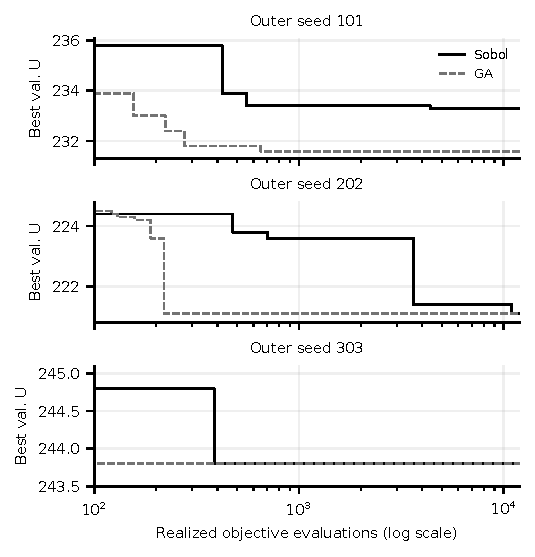
\includegraphics[width=\columnwidth]{figures/optimizer_anytime.pdf}
\caption{Validation-only replay: best observed loss versus realized objective calls for each outer partition. Duplicate GA evaluations count toward the budget. All final vectors match the frozen run.}
\label{fig:anytime}
\end{figure}

\begin{table}[t]
\caption{Mean workflow decision counts (GB-18). $R_+$ denotes positive REVIEW; total REVIEW also contains negatives.}
\label{tab:counts}
\centering
\begin{tabular}{lrrrr}
\toprule
Policy & FP & FN & $R_+$ & REVIEW\\
\midrule
B0 & 88.0 & 2171.3 & 160.7 & 168.7\\
B1 & 115.3 & 1557.7 & 430.0 & 762.3\\
B2 & 107.7 & 1560.3 & 509.7 & 843.7\\
B3 & 107.7 & 1557.7 & 513.3 & 852.3\\
Chow & 96.0 & 1281.0 & 890.3 & 4060.3\\
\bottomrule
\end{tabular}
\end{table}

\textbf{Candidate ceiling.} The 3,312 blocking-missed positives impose an 88.6742\% global retrieval ceiling. In sealed roles the missed counts are 1,034, 1,014, and 1,007. Counting them as workflow FN prevents model-scored metrics from overstating end-to-end recall.

\section{Limitations and Threats to Validity}
The study uses one historical corpus and three deterministic outer partitions, so it does not establish external generalization. Candidate blocking creates a fixed retrieval ceiling and possible selection effects. The model-family screen is historical development evidence and is not directly comparable with the authoritative protocol. The semantic intervention is only one fixed cosine; URL/domain evidence considered during broader development is not part of the final 17-feature schema.

The objective coefficients are assumed remediation effort, not measured economic cost; a different preference can select another operating point. REVIEW is an offline output, with no evaluation of human accuracy, workload, agreement, or latency. Pairwise MATCH decisions need not be transitive; no entity-clustering consistency was evaluated. Missing-name comparisons yield zero similarity rather than evidence of identity. Exact username/URL matching is a deterministic heuristic, not proof of shared identity. GA does not consistently beat equal-budget Sobol, and the direct-risk baseline is competitive. Calibration-quality diagnostics and an independent replication corpus are absent. Finally, public hosting was verified, but reuse license, redistribution permission, collection/Terms-of-Service evidence, consent, and ethics documentation were not; release should remain limited to code, configurations, hashes, and aggregates pending clarification.

\section{Conclusion}
Cross-platform identity resolution requires both heterogeneous evidence integration and operational decision control. Empirical development motivated a multi-feature Gradient Boosting scorer; the authoritative ablation finds little additional benefit from one MiniLM cosine. Validation-selected three-way operation lowers declared loss relative to fixed thresholds. Its decision-conditional F1 improvement is larger than its automatic end-to-end gain and depends partly on increased deferral. Genetic search can select the expanded policy, but its outcome is similar to equal-budget Sobol and to the closed-form posterior-risk baseline. The evidence supports a reproducible comparison of profile-linkage operating points, with explicit review burden and candidate-retrieval limits.

\bibliographystyle{IEEEtran}
\bibliography{references}
\end{document}
